%!TEX root = ../Dimensionieren I.tex

\section{Allgemeines} % (fold)
	Beziehungen zwischen Verschiebungen und Dehnungen:
	\begin{equation*}
		\varepsilon_x = \frac{\partial u}{\partial x}, \quad \varepsilon_\vartheta = \frac{1}{r} \frac{\partial v}{\partial r} + \frac{w}{r}, \quad \varepsilon_r = \frac{\partial w}{\partial r}
	\end{equation*}
	\begin{equation*}
		\gamma_{\vartheta r} = \frac{\partial v}{\partial r} + \frac{1}{r}\frac{\partial w}{\partial \vartheta} - \frac{v}{r}, \quad \gamma_{rx} = \frac{\partial w}{\partial x} + \frac{\partial u}{\partial r}, \quad \gamma_{x\vartheta} = \frac{\partial v}{\partial x} + \frac{1}{r}\frac{\partial u}{\partial \vartheta}
	\end{equation*}
	\begin{equation*}
		\omega = \frac{v}{r}, \quad P = M \cdot \omega
	\end{equation*}
	
	\subsection{Hooke'sches Gesetz} % (fold)
		\begin{equation*}
			\varepsilon_x = \frac{1}{E}[\sigma_x - \nu (\sigma_\vartheta + \sigma_r)]
		\end{equation*}
		\begin{equation*}
			\varepsilon_\vartheta = \frac{1}{E}[\sigma_\vartheta - \nu (\sigma_x + \sigma_r)]
		\end{equation*}
		\begin{equation*}
			\varepsilon_r = \frac{1}{E}[\sigma_r - \nu (\sigma_\vartheta + \sigma_x)]
		\end{equation*}
	% subsection: Hooke'sches Gesetz (end)
	\subsection{Ebener Verformungszustand (EFZ)} % (fold)
		Verschiebungsdifferentialgleichung:
		\begin{equation*}
			w_{rr} + \frac{1}{r}w_r - \frac{1}{r^2}w + \frac{1-2\nu-2\nu^2}{(1-\nu)E}\rho r \omega^2 = 0
		\end{equation*}
	% subsection: Ebener Verformungszustand (EFZ) (end)
	\subsection{Ebener Spannungszustand (ESZ)} % (fold)
		\begin{equation*}
			w_{rr} + \frac{1}{r}w_r - \frac{1}{r^2}w + \frac{1-\nu^2}{E}\rho r \omega^2=0
		\end{equation*}
	% subsection: Ebener Spannungszustand (ESZ) (end)
	\subsection{Lösung} % (fold)
		Allgemein für Rohrquerschnitte:
		\begin{equation*}
			w_H(r) = ar + \frac{b}{r}
		\end{equation*}
		Für Vollquerschnitte:
		\begin{equation*}
			w_H(r) = ar
		\end{equation*}
	% subsection: Lösung (end)
% section: Allgemeines (end)
\section{Dickwandiger Zylinder} % (fold)
	\begin{flushright}
		\vspace{-1cm}
		$\displaystyle\parens{\frac{r_m}{t} < 100}$
		\vspace{0cm}
	\end{flushright}
	\begin{equation*}
		\varepsilon_\vartheta = a + \frac{1}{r^2}b, \quad \varepsilon_r = a - \frac{1}{r^2}b
	\end{equation*}
	
	\subsection{Druckbehälter mit freier Längsdehnung} % (fold)
		\begin{equation*}
			\sigma_x = 0, \quad \sigma_r (r_i) = - p_i, \quad \sigma_r (r_a) = - p_a
		\end{equation*}
		\begin{equation*}
			\sigma_\vartheta = A + \frac{B}{r^2}, \quad \sigma_r = A - \frac{B}{r^2}, \quad \sigma_x = C
		\end{equation*}
	% subsection: Druckbehälter mit freier Längsdehnung (end)
	\subsection{Druckbehälter mit behinderter Längsdehnung} % (fold)
		\begin{equation*}
			\sigma_r (r_i) = - p_i, \quad \sigma_r (r_a) = - p_a
		\end{equation*}
		\begin{equation*}
			\sigma_\vartheta = A^* + \frac{B^*}{r^2}, \quad A^* - \frac{B^*}{r^2}
		\end{equation*}
	% subsection: Druckbehälter mit behinderter Längsdehnung (end)
	\subsection{Vergleichsspannung} % (fold)
		Maximum bei $r_i$:
		\begin{equation*}
			\sigma_{\text{V}} = \sigma_\vartheta - \sigma_r
		\end{equation*}
		\begin{equation*}
			S_F = \frac{\sigma_S}{\sigma_V} = \frac{\sigma_S}{\sigma_\vartheta - \sigma_r}
		\end{equation*}
		Dabei tritt $S_{F\text{, max}}$ jeweils am inneren Radius auf.
	% subsection: Vergleichsspannung (end)
% section: Dickwandiger Zylinder (end)
\section{Dünnwandiger Zylinder} % (fold)
	\begin{wrapfigure}[0]{r}{.65\columnwidth}
		\vspace{-1cm}
		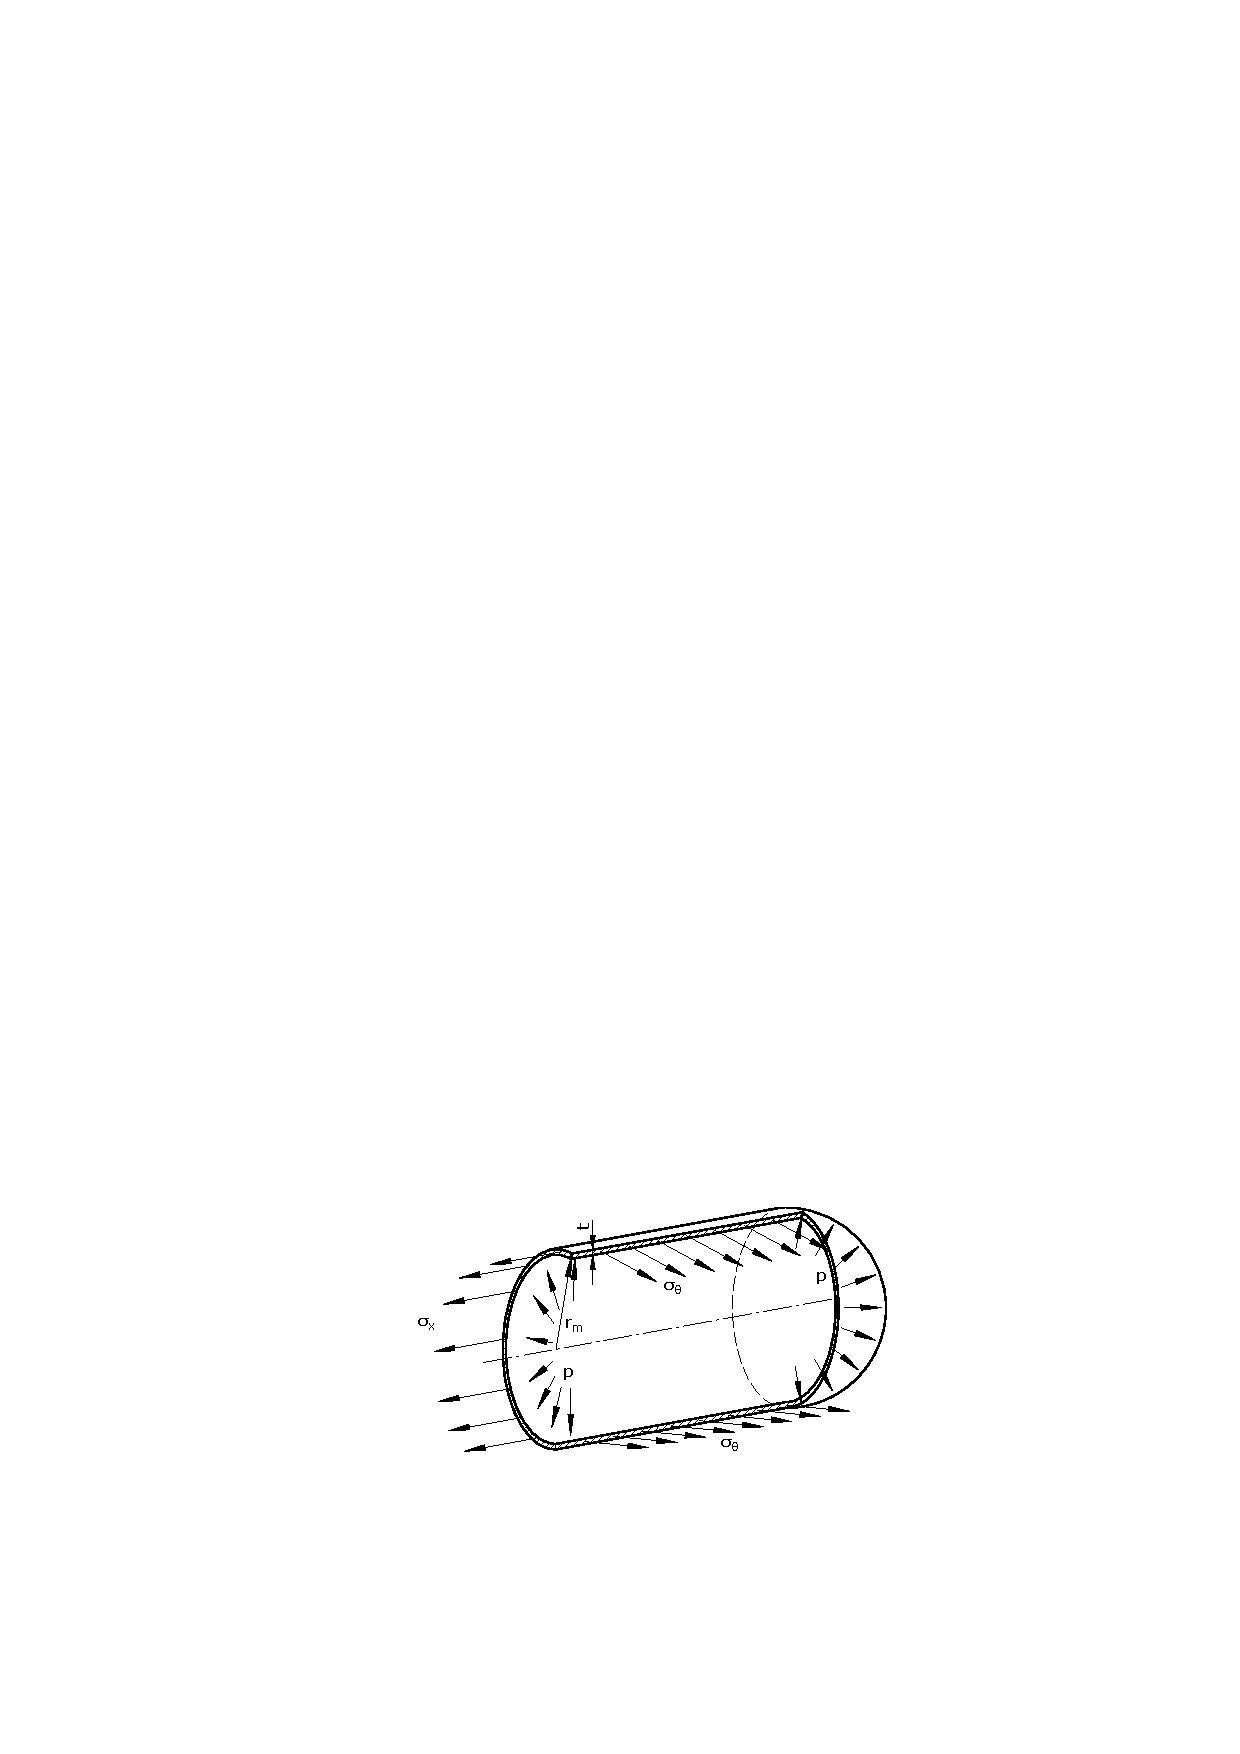
\includegraphics[width=.65\columnwidth]{graphics/duennwandig}
	\end{wrapfigure}
	{
		\setlength{\mathindent}{.5\mathindent}
		\begin{align*}
			\sigma_\vartheta &= \frac{r_m}{t}(p_i - p_a) \\
			\sigma_x &= \frac{r_m}{2t}(p_i-p_a)
		\end{align*}
	}
% section: Dünnwandiger Zylinder (end)
\section{Rotierender Zylinder} % (fold)
	\begin{equation*}
		\sigma_\vartheta = \frac{E}{1-\nu^2}\left[ a(1+\nu) + \frac{b \cdot (1-\nu)}{r^2}\right] - r^2 \frac{\rho \omega^2}{8}(1+3\nu)
	\end{equation*}
	\begin{equation*}
		\sigma_r = \frac{E}{1-\nu^2}\left[ a(1+\nu) + \frac{b \cdot (1-\nu)}{r^2}\right] - r^2 \frac{\rho \omega^2}{8}(3+\nu)
	\end{equation*}
	
	\subsection{Schwungscheibe ohne Bohrung} % (fold)
		\begin{equation*}
			a = \frac{(1-\nu)(3+\nu)}{E}\cdot r_a^2\cdot \frac{\rho\omega^2}{8}, \quad b=0
		\end{equation*}
		\begin{equation*}
			\sigma_\vartheta = \frac{\rho \omega^2}{8}\left[ (3+\nu)\cdot r_a^2 - (1+3\nu)\cdot r^2\right]
		\end{equation*}
		\begin{equation*}
			\sigma_r = \frac{\rho \omega^2}{8} \left[ (3+\nu)(r_a^2 - r^2)\right]
		\end{equation*}
		\begin{equation*}
			w = \frac{\rho \omega^2}{8}\left[ (3+\nu)\cdot r_a^2 - (1+\nu)\cdot r^2\right](1-\nu)r
		\end{equation*}
	% subsection: Schwungscheibe ohne Bohrung (end)
	\subsection{Schwungscheibe mit Bohrung} % (fold)
		\begin{equation*}
			\sigma_\vartheta = \frac{\rho \omega^2}{8} \left[ (3+\nu)\left( r_i^2 +r_a^2 + \frac{r_i^2 r_a^2}{r^2}\right) - (1 + 3\nu)r^2\right]
		\end{equation*}
		\begin{equation*}
			\sigma_r =  \frac{\rho \omega^2}{8} (3+\nu) \left[ r_i^2 + r_a^2 - \frac{r_i^2r_a^2}{r^2} - r^2\right]
		\end{equation*}
	% subsection: Schwungscheibe mit Bohrung (end)
% section: Rotierender Zylinder (end)
